% vim: tw=80

\chapter{PDF Constraints of the triple-differential Dijet Measurement}

In many precision measurements at the LHC, the proton PDFs are an essential
ingredient. As the PDFs cannot be calculated from perturbative QCD, they are
derived from experimental data of collider and fixed-target experiments.
Deep-inelastic scattering (DIS) data from the HERA collider cover most of the
kinematic phasespace. The triple-differential dijet cross section contains
additional information in the high-$x$ region and can constrain the PDFs, in
particular the gluon PDF. 


% The HERAFitter project~\cite{Aaron:2009kv,Aaron:2009aa,HERAFitter:2013hf} is an open
% source fitting framework designed to derive PDFs from data. It has a
% modular structure, encompassing a variety of theoretical predictions
% for different processes and phenomenological approaches for the PDF
% determination. Confronting data with theoretical predictions the
% parton distributions are determined.  In this study HERAFitter is
% employed to estimate the impact of the CMS inclusive jet data on the
% PDFs and their uncertainties using the fixed-order theory predictions
% and NP corrections as defined in the previous section.



\begin{figure}[tbp]
  \centering
  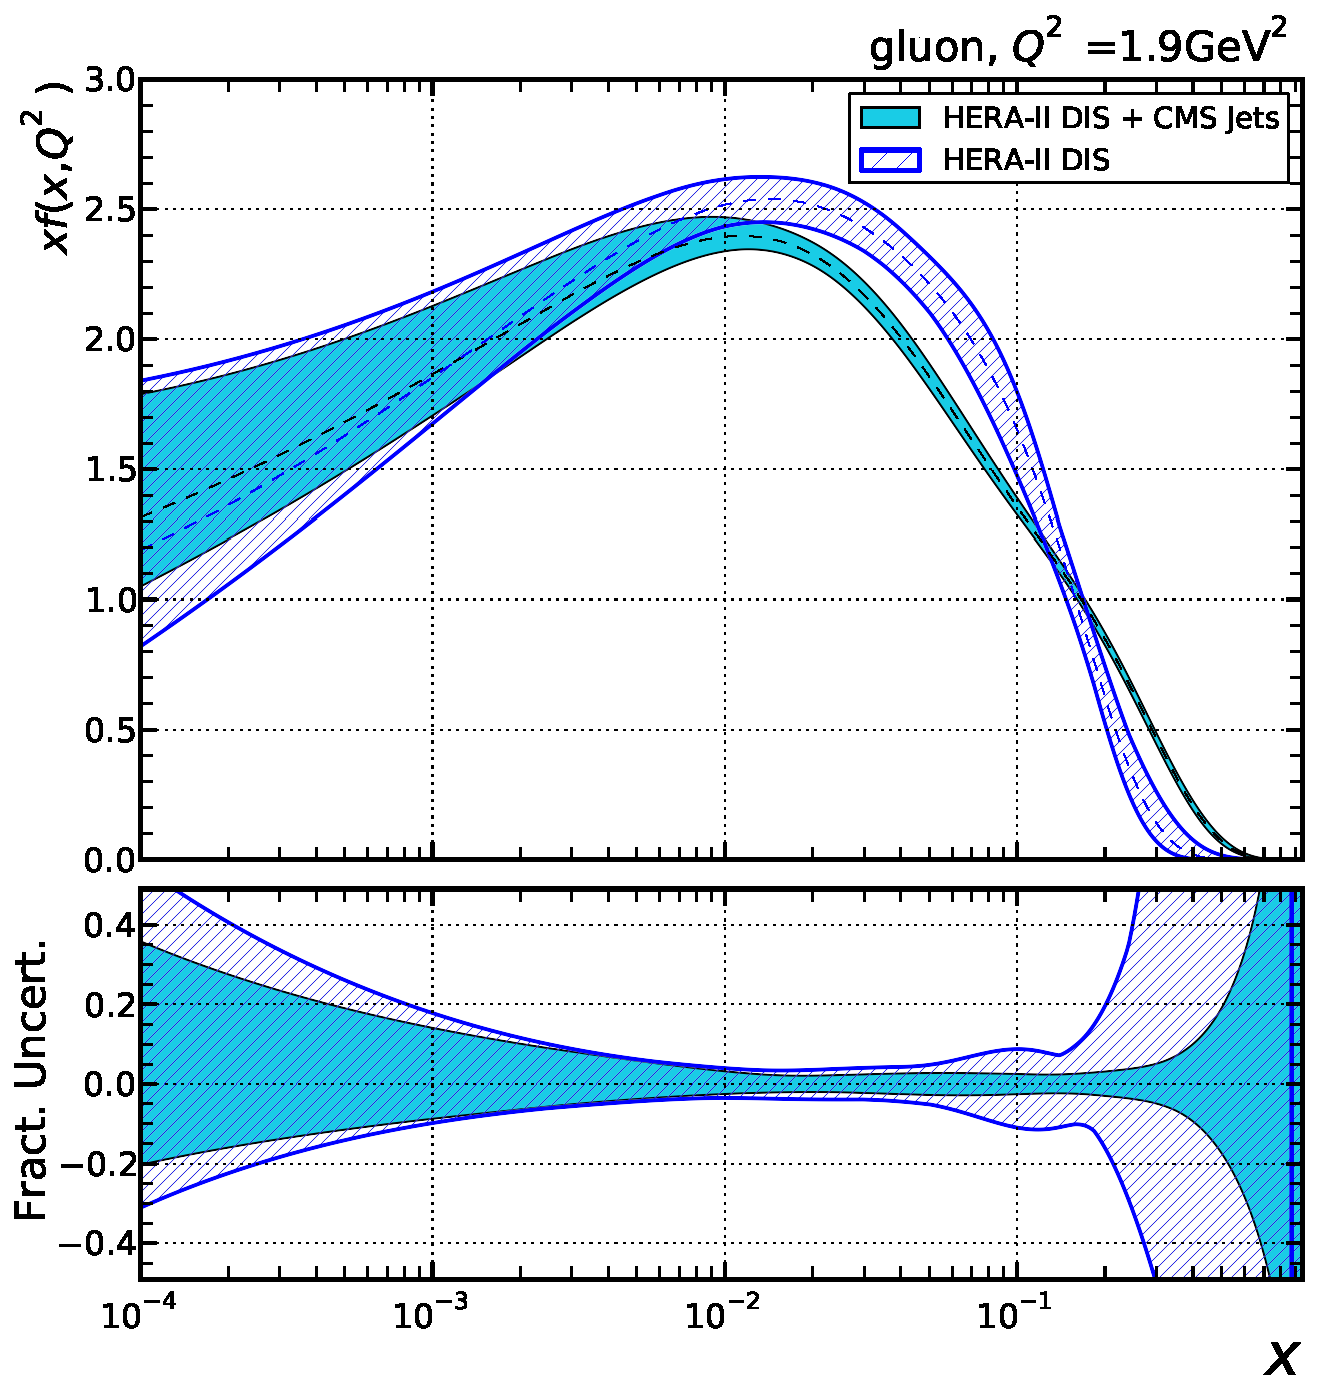
\includegraphics[width=0.48\textwidth]{figures/pdf_constraints/direct/HFTD_HERACMSTDJETS_V017_EIG_0_1_9.pdf}\hfill%
  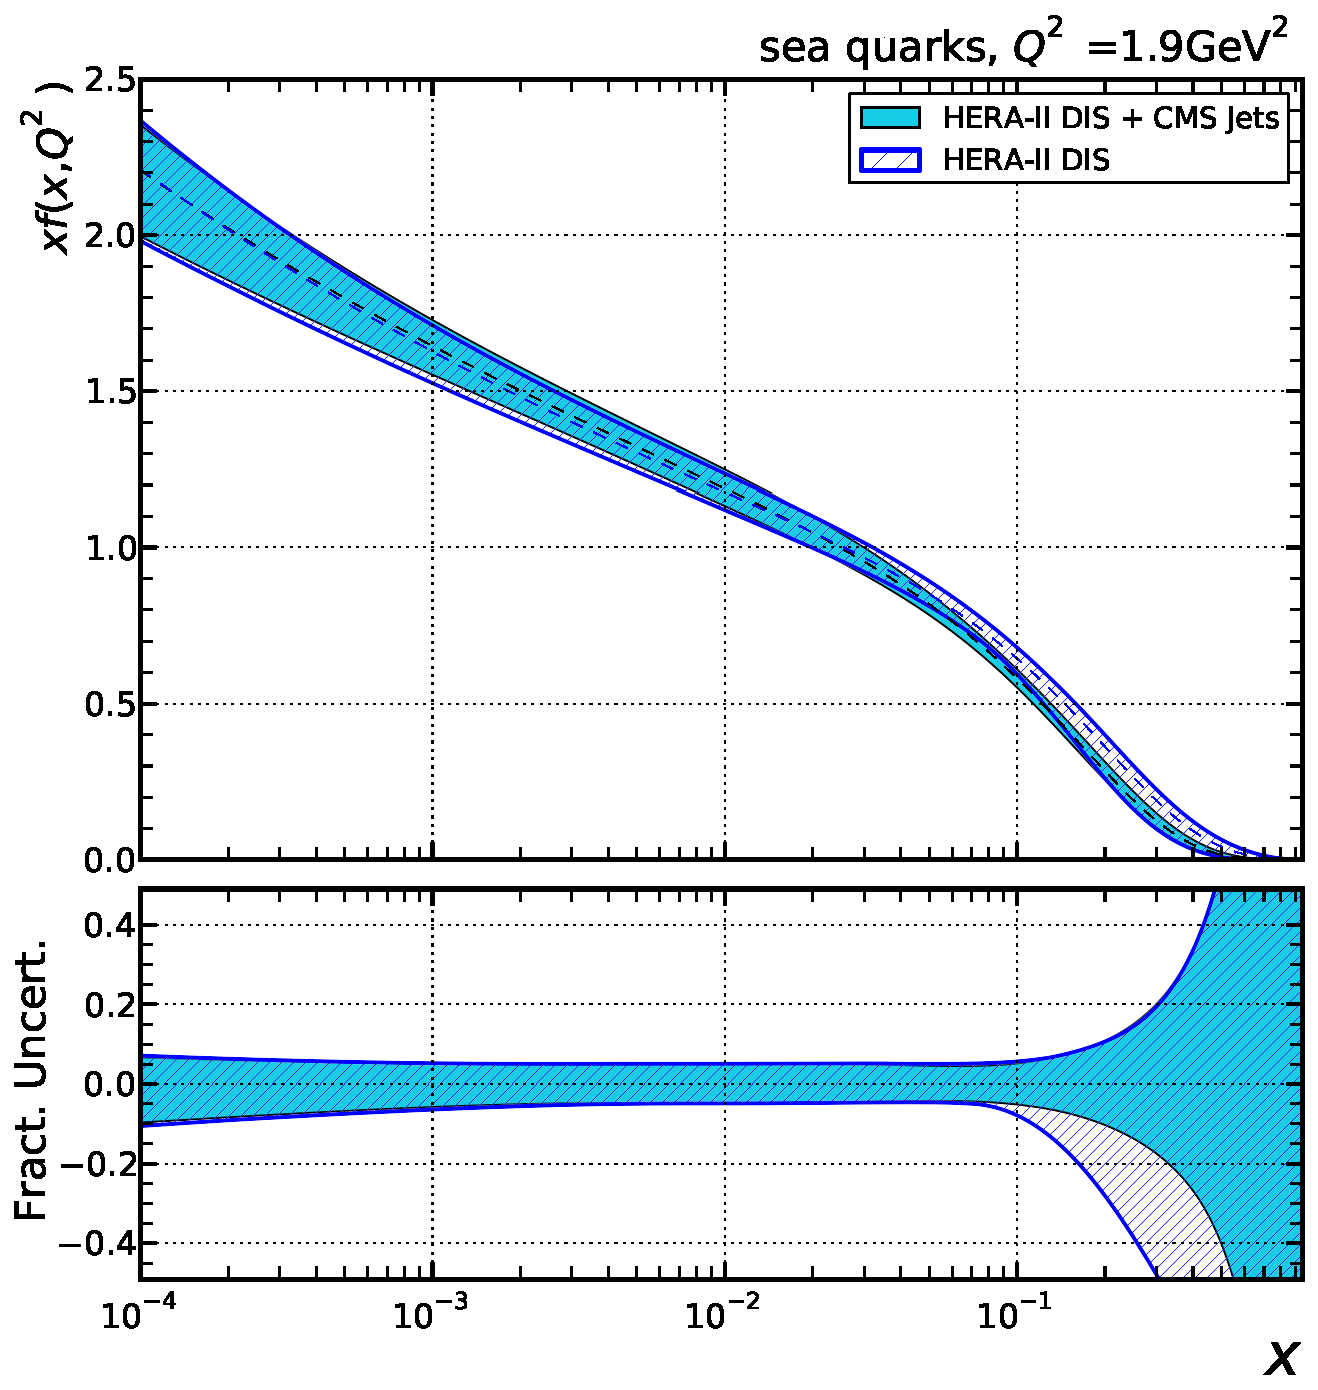
\includegraphics[width=0.48\textwidth]{figures/pdf_constraints/direct/HFTD_HERACMSTDJETS_V017_EIG_9_1_9.pdf}
  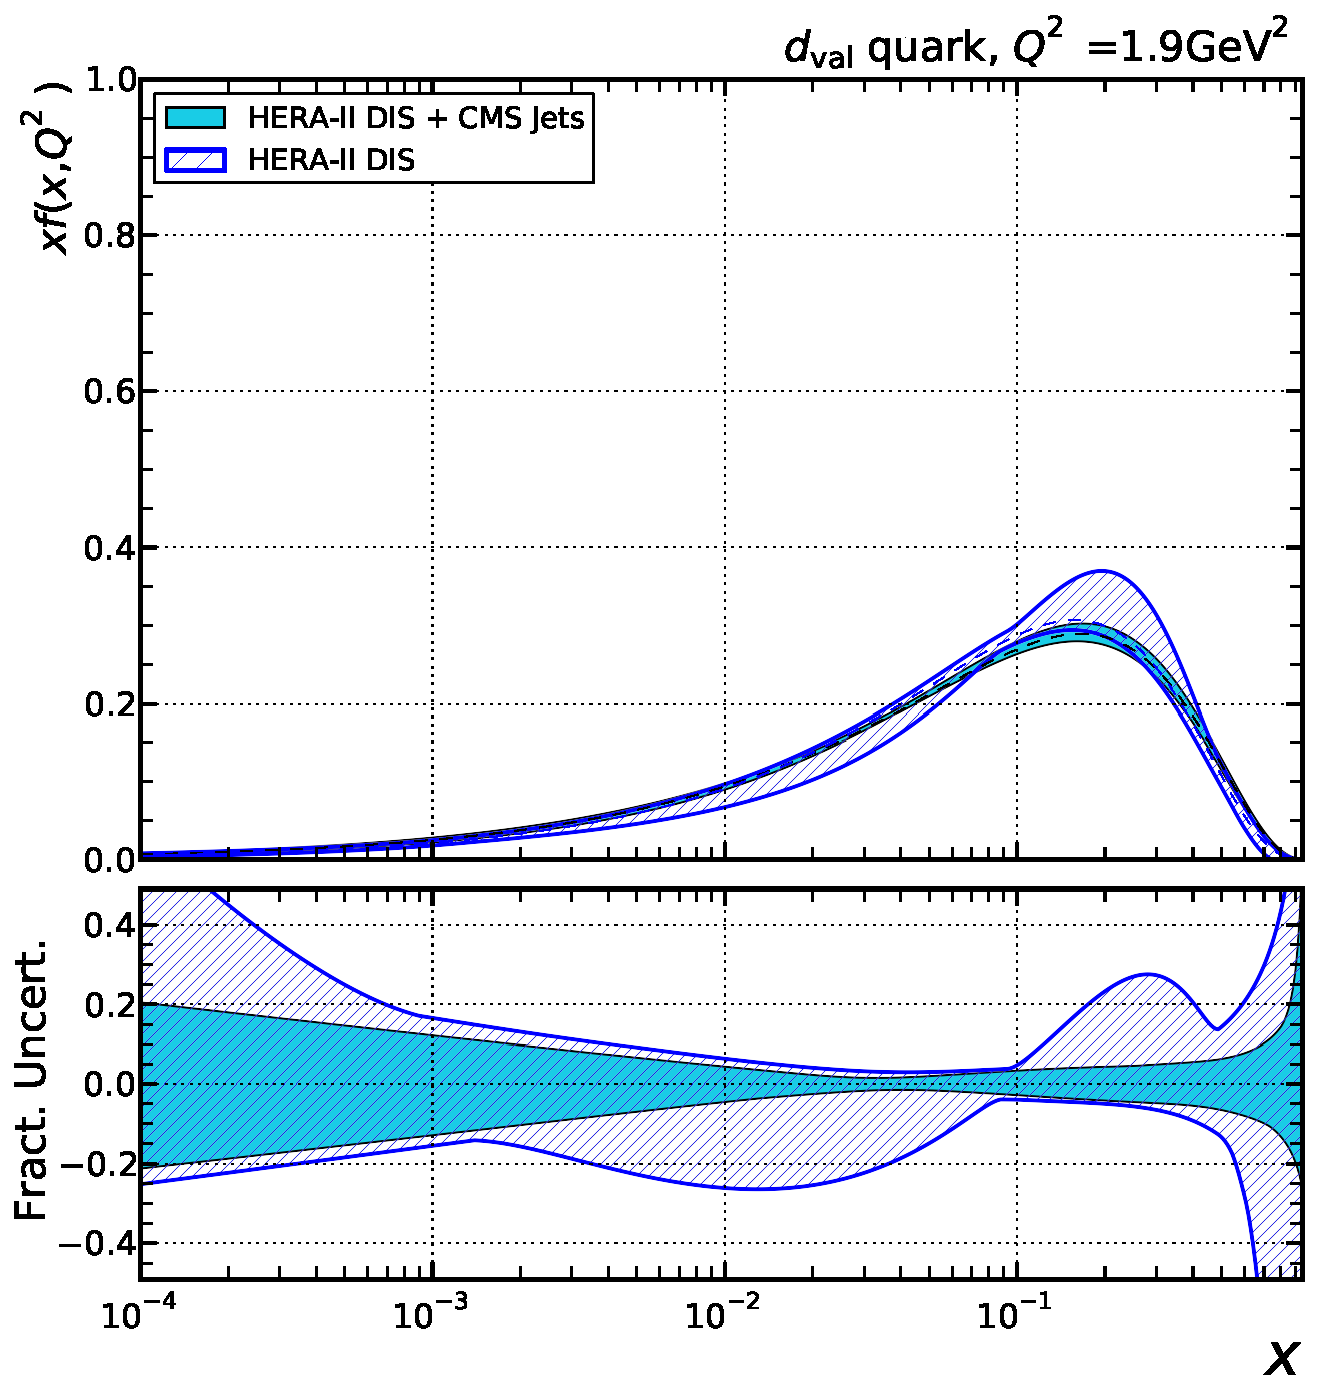
\includegraphics[width=0.48\textwidth]{figures/pdf_constraints/direct/HFTD_HERACMSTDJETS_V017_EIG_7_1_9.pdf}\hfill%
  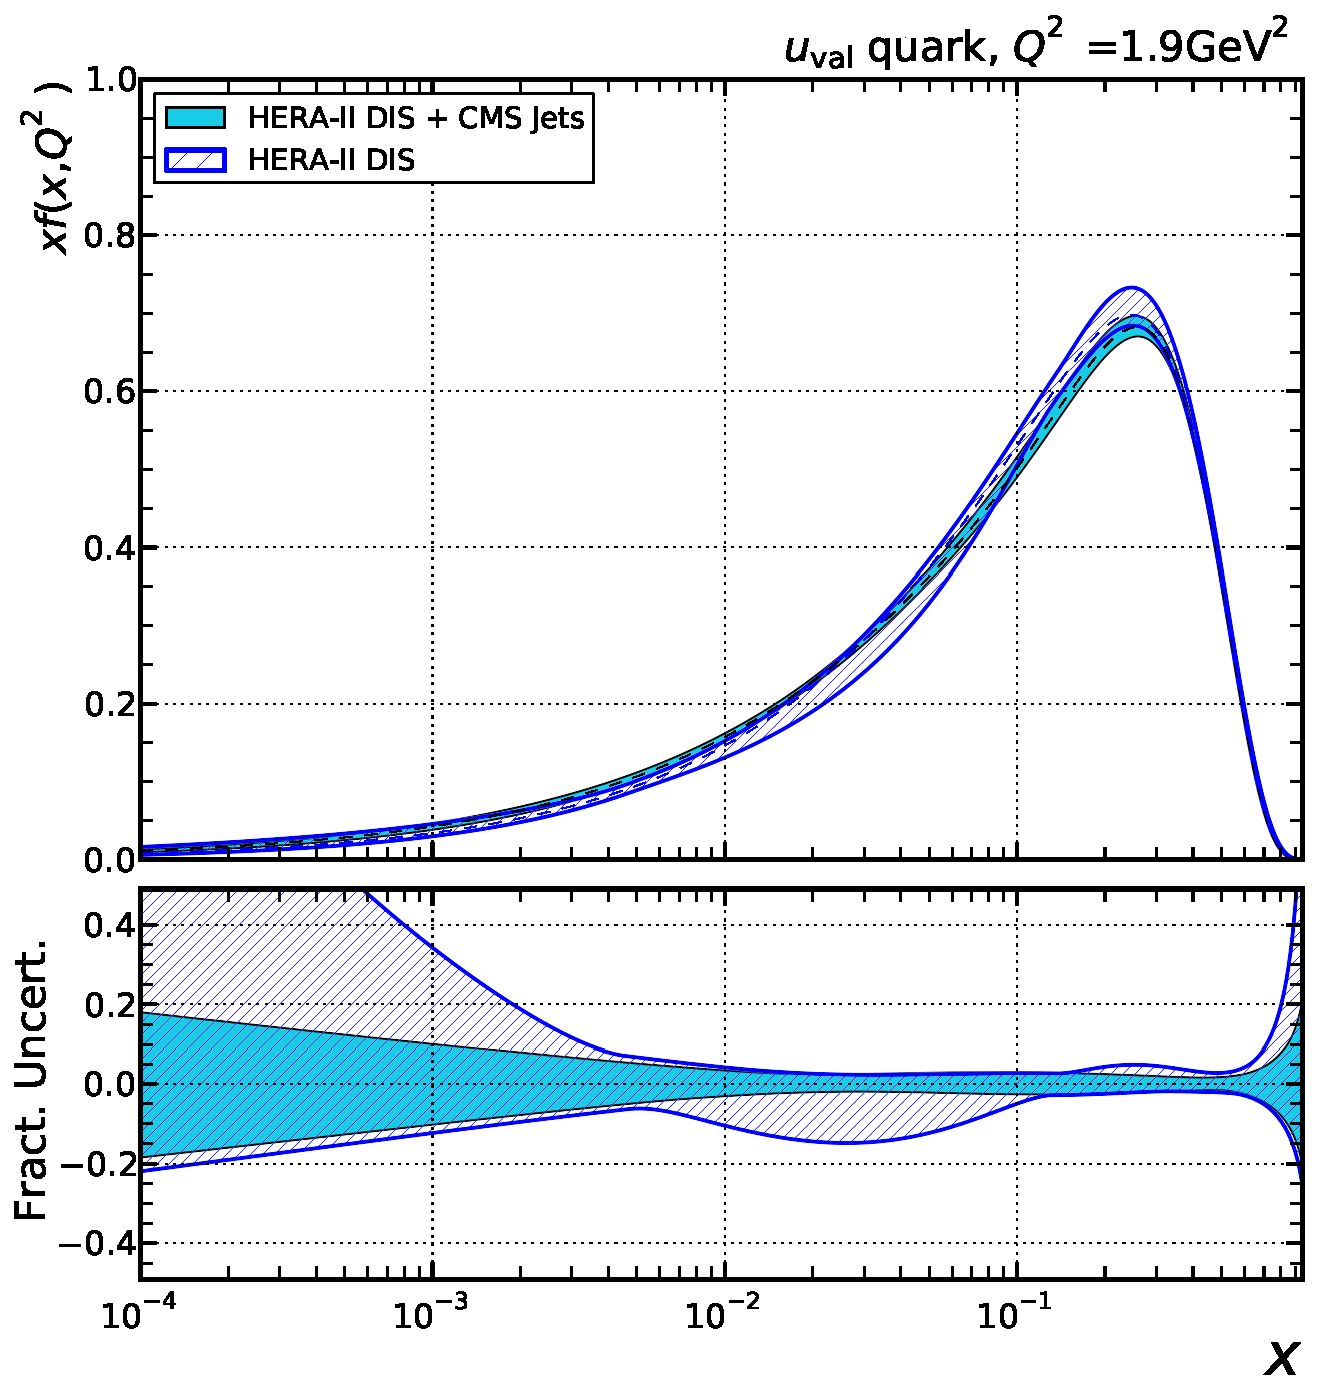
\includegraphics[width=0.48\textwidth]{figures/pdf_constraints/direct/HFTD_HERACMSTDJETS_V017_EIG_8_1_9.pdf}
  \caption{}
  \label{fig:pdfconstraints:direct:19}
\end{figure}



\section{Sensitivity of PDFs to Dijet Measurement}
\label{sec:pdf_sensitivity}

% The potential impact of the CMS inclusive jet data can be illustrated
% by the correlation between the inclusive jet cross section
% $\sigma_{\mathrm{jet}}(x,Q^2)$ and the PDF $xf_i(x,Q^2)$ for each
% parton of flavour $i$. As before, $x$ is the fraction of the proton
% momentum, and $Q$ is the relevant energy scale of the hard process,
% which in the case of inclusive jets is identified with the jet \pt.
%
% The NNPDF Collaboration~\cite{Ball:2008by} provides PDF sets in the
% form of an ensemble of PDFs called replicas, which sample variations
% in the PDF parameter space allowed within uncertainties. Evaluating
% means and variance with the help of these replicas, predictions
% including uncertainties are derived for PDF dependent observables.
% For an NNPDF ensemble with $N_{\mathrm{rep}}$ replicas, the
% correlation coefficient $\varrho$ between a cross section and the PDF
% for flavour $i$ is then defined as:
%
% \begin{equation}
%   \varrho_i \left[ \sigma_{\mathrm{jet}}(x,Q^2) , xf_i(x,Q^2) \right] =
%   \frac{N_{\mathrm{rep}}}{(N_{\mathrm{rep}}-1)} \frac{\langle
%     \sigma_{\mathrm{jet}}(x,Q^2) xf_i(x,Q^2) \rangle -
%     \langle \sigma_{\mathrm{jet}} \rangle \langle xf_i(x,Q^2)
%     \rangle}{\Delta_{\sigma_{\mathrm{jet}}(x,Q^2)} \Delta_{xf_i(x,Q^2)}}\,.
% \end{equation}
%
% Here, the uncertainties of the jet cross sections and the PDFs
% themselves are represented by $\Delta_{\sigma_\mathrm{jet}}$ and
% $\Delta_{xf(x,Q^2)}$, respectively.
% Figure~\ref{fig:correlation_pdf_xs_gqq} presents the correlation
% coefficient between the inclusive jet cross section and the gluon, up,
% and down quark PDFs in the proton.
%
% \begin{figure}[h!tb]
%   \centering
%   \includegraphics[width=0.45\textwidth]{herafitter_Figures/correlation_plots/corr_fnl2332d_NNPDF21_gluon_y0_0_bw}\hfill%
%   \includegraphics[width=0.45\textwidth]{herafitter_Figures/correlation_plots/corr_fnl2332d_NNPDF21_gluon_y2_0_bw}
%   \includegraphics[width=0.45\textwidth]{herafitter_Figures/correlation_plots/corr_fnl2332d_NNPDF21_u_quark_y0_0_bw}\hfill%
%   \includegraphics[width=0.45\textwidth]{herafitter_Figures/correlation_plots/corr_fnl2332d_NNPDF21_u_quark_y2_0_bw}
%   \includegraphics[width=0.45\textwidth]{herafitter_Figures/correlation_plots/corr_fnl2332d_NNPDF21_d_quark_y0_0_bw}\hfill%
%   \includegraphics[width=0.45\textwidth]{herafitter_Figures/correlation_plots/corr_fnl2332d_NNPDF21_d_quark_y2_0_bw}
%   \caption{The correlation coefficient between the inclusive jet cross
%     section and the gluon (top row), the up quark (middle row), and
%     the down quark PDF (bottom row) as a function of the momentum
%     fraction $x$ of the proton and the momentum scale $Q$ of the hard
%     process. The correlation is shown for the central rapidity region
%     $|y|<0.5$ (left) and for $2.0<|y|<2.5$ (right).}
%   \label{fig:correlation_pdf_xs_gqq}
% \end{figure}
%
% The correlation between the gluon PDF and the inclusive jet cross
% section is observed to be largest at central rapidity for all jet
% transverse momenta. In contrast the correlation between the quark
% distributions and the jet cross section is rather small in this
% kinematic region such that a large impact on the quark distribution is
% not expected from including these jet data into PDF fits. In the
% forward region though the correlation between the quark distributions
% and the jet cross sections increases with $x$ at high \pt. In summary,
% a significant reduction of the PDF uncertainties is expected by
% including the CMS inclusive jet cross section into fits of the proton
% structure.

\section{Setup of the HERAFitter fitting framework}
\label{section:herafittersetup}

% In the following the impact of the CMS inclusive jet data on proton
% PDFs is investigated by including the jet cross section measurement
% into a combined fit with the HERA inclusive DIS cross
% sections~\cite{Aaron:2009aa}, which were the basis for the
% determination of the HERAPDF1.0 PDF set.
%
% The analysis is performed within the HERAFitter framework, which is
% based on the Dokshitzer-Gribov-Lipatov-Altarelli-Parisi
% (DGLAP)~\cite{Gribov:1972ri,Altarelli:1977zs,Dokshitzer:1977sg}
% evolution scheme at NLO as implemented in the QCDNUM
% package~\cite{Botje:2010ay}. DIS data in the fit are required to have
% $Q^2 > Q_\mathrm{min}^2 = 3.5 \GeVsq$ to ensure the applicability of
% perturbative QCD\@. The following PDFs are assumed to be independent
% in the fit procedure: $xu_v(x)$, $xd_v(x)$, $xg(x)$, and
% $x\bar{U}(x)$, $x\bar{D}(x)$, where $x\bar{U}(x) = x\bar{u}(x)$, and
% $x\bar{D}(x) = x\bar{d}(x) + x\bar{s}(x)$. A parameterization with 13
% free parameters is used, similar to Ref.~\cite{Abramowicz:1900rp}. At
% the starting scale $Q_0$ of the QCD evolution, chosen to be $Q_0^2 =
% 1.9 \GeVsq$, the PDFs are parameterized as follows:
%
% \begin{align}
%   xg(x) &= A_g x^{B_g} (1-x)^{C_g} - A'_g x^{B'_g} (1-x)^{C'_g} \\
%   xu_v(x) &= A_{u_{v}} x^{B_{u_{v}}} (1-x)^{C_{u_{v}}} (1 + E_{u_{v}}x^2)\\
%   xd_v(x) &= A_{d_v} x^{B_{d_v}} (1-x)^{C_{d_{v}}}\\
%   x\bar U(x) &= A_{\bar U} x^{B_{\bar U}} (1-x)^{C_{\bar U}}\\
%   x\bar D(x) &= A_{\bar D} x^{B_{\bar D}} (1-x)^{C_{\bar D}}
% \end{align}
%
% The normalization parameters $A_g$, $A_{u_{v}}$ and $A_{d_{v}}$ are
% constrained by QCD sum rules. Additional constraints $B_{\bar
%   U}=B_{\bar D}$ and $A_{\bar U} = A_{\bar D}(1-f_s)$ are applied to
% ensure the same normalization for the $\bar u$ and $\bar d$ densities
% for $x \rightarrow 0$. The strangeness fraction is set to $f_s =
% 0.31$, as obtained from neutrino-induced di-muon
% production~\cite{Mason:2007zz}. The parameter $C'_g$ is fixed to
% 25~\cite{Martin:2009iq,Thorne:2006qt}. A generalized-mass variable
% flavour number scheme~\cite{Thorne:1997ga,Thorne:2006qt} is used with
% the strong coupling constant set to $\alpsmz= 0.1176$.


\subsection{Determination of PDF uncertainties in the HERAFitter framework}
\label{section:treatment_pdf_uncertainties}

% The uncertainty of the PDFs is subdivided into experimental, model,
% and parameterization uncertainties, which are studied
% separately. Experimental uncertainties result from the propagated
% statistical and systematic uncertainties of the input data.
% For the model uncertainties the following variations of
% model assumptions are considered:
%
% \begin{itemize}
% \item The strangeness fraction $f_s$, by default equal to $0.31$, is
%   varied between $0.23$ and $0.38$.
% \item The b-quark mass is varied by $\pm 0.25\GeV$ around the central
%   value of $4.75\GeV$.
% \item The minimum $Q^2$ value for data used in the fit,
%   $Q^2_\mathrm{min}$, is varied from $Q^2_\mathrm{min} = 3.5\GeVsq$ to
%   $5.0\GeVsq$. For the variation fit with $Q_{\mathrm{min}}^2 = 5.0
%   \GeVsq$, the parameter $B_{g}'$ is fixed to the value obtained in
%   the central fit.
% \end{itemize}
%
% The parameterization uncertainty is estimated as described in
% Ref.~\cite{Aaron:2009aa}. Employing the more general form of
% parameterization
%
% \begin{align}
%   xg(x) &= A_g x^{B_g} (1-x)^{C_g} (1  + D_g x + E_g x^2) - A'_g x^{B'_g} (1-x)^{C'_g};\\
%   xf(x) &= A_{f}  x^{B_{f}} (1-x)^{C_{f}} (1 + D_{f}x + E_{f}x^2)
% \end{align}
%
% it is tested successively whether the inclusion of additional fit
% parameters leads to a variation in the shape of the fitted results.
% Furthermore, the starting scale $Q_0$ is changed to $Q^2_0 =
% 1.5\GeVsq$ and $Q^2_0 = 2.5\GeVsq$.  The maximal deviations of the
% resulting PDFs from those obtained in the central fit define the
% parameterization uncertainty. The experimental, model, and
% parameterization uncertainties are added in quadrature to give the
% final PDF uncertainty.
%

\subsection{Definition of the goodness-of-fit estimator}
\label{sec:fitsetup}

% The agreement between data points $D_i$ and the theoretical
% predictions $T_i$ is estimated via a least-squares method. All $K$
% fully correlated sources of systematic uncertainty $\beta_{k}$ are
% treated using nuisance parameters $r_k$ and are assumed to be
% multiplicative to avoid the statistical bias that arises from
% uncertainty estimations taken from data~\cite{Lyons:1989gh}.
% % in order to avoid the d'Agostini bias~\cite{D'Agostini:2003nk}.
% As a consequence the covariance matrix,
% defined as $\mathrm{C} = \mathrm{cov}_{\mathrm{stat}} +
% \mathrm{cov}_{\mathrm{uncor}}$, has to be reevaluated in each
% iteration step.
%
% To inhibit the compensation of large systematic shifts by increasing
% the theory prediction and the statistical uncertainties at the same
% time, the systematic shifts of the theory are taken into account
% before the rescaling of the statistical uncertainty. Otherwise
% alternative minima in \chisq, which is defined as
%
% \begin{equation}
%   \chi^2 = \sum_{ij}^N \left(D_i - T_i - \sum_k^K r_k \beta_{ik}\right) \mathrm{C}_{ij}^{-1}
%   \left(D_j - T_j - \sum_k^K r_k \beta_{jk} \right) + \sum_k^K r_k^2\,,
%   \label{chi2_nuisance}
% \end{equation}
%
% could be found that are associated to a high theory prediction with at
% the same time large shifts (pulls) for the nuisance parameters. This
% is clearly undesirable~\cite{HERAFitter:2013hf}.


\subsection{Treatment of CMS data uncertainties}
\label{section:cmsdatauncertainties}

% The jet energy scale is the dominant source of experimental systematic
% uncertainty on jet cross sections. As described in
% Section~\ref{sec:measurementjec}, the \pt and $\eta$ dependent jet
% energy scale uncertainties are split into 16 uncorrelated sources
% which are fully correlated among themselves. Following the modified
% recommendation for the correlations versus rapidity of the
% \textsc{Single Pion} source as given in
% Section~\ref{sec:measurementjec}, it is necessary to split this source
% into five parts for the purpose of using the uncertainties published
% in~\cite{CMS-PAPERS-QCD-11-004} within the \chisq fits. The complete
% setup including other uncertainties is shown in
% Table~\ref{tab:cmsjets2011:nuisance}.
%
% Employing the technique of nuisance parameters, the impact of each
% systematic source of uncertainty on the fit result can be examined
% separately. In case of an adequate estimation of the size and the
% correlations of all uncertainties it is expected that the majority of
% all systematic sources are shifted by less than one standard deviation
% $\sigma$ from the default in the fitting procedure.
% Table~\ref{tab:cmsjets2011:nuisance} demonstrates that this is the
% case for the CMS jet data with the described procedure.
%
% \begin{table}[htbp]
%   \caption{19 independent sources of systematic uncertainty are considered in the
%     CMS inclusive jet measurement. Out of these 16 are related to the JES
%     and are listed first. In order to implement the improved correlation
%     treatment as described in Section~\ref{sec:measurementjec}, the
%     \textsc{SinglePion} source, see also the
%     Appendix~\ref{sec:jessources}, has been split up into five
%     sources. The shift from the default value in each source of systematic
%     uncertainty is determined by nuisance parameters in the fit and is
%     presented in units of standard deviations.}
%   \label{tab:cmsjets2011:nuisance}
%   \centering
%   \begin{tabular}{lrlr}
%     \hline\hline
%     Systematic source         & Shift in $\sigma$ & Systematic source & Shift in $\sigma$\rbthm\\\hline\hline
%     \textsc{Absolute}         & -0.20 &   \textsc{RelativeJEREC2}   & -0.28\rbtrr\\
%     \textsc{HighPtExtra}      & -0.60 &   \textsc{RelativeJERHF}    &  0.00\rbtrr\\
%     \textsc{SinglePionBarrel} &  0.64 &   \textsc{RelativeStatEC2}  & -0.28\rbtrr\\
%     \textsc{SinglePionEndcap} & -1.64 &   \textsc{RelativeStatHF}   &  0.00\rbtrr\\
%     \textsc{SinglePionY0005}  & -0.10 &   \textsc{RelativeFSR}      & -0.01\rbtrr\\
%     \textsc{SinglePionY0510}  &  0.12 &   \textsc{PileUpDataMC}     &  0.69\rbtrr\\
%     \textsc{SinglePionY1015}  &  0.85 &   \textsc{PileUpOOT}        & -0.09\rbtrr\\
%     \textsc{Flavor}           &  0.21 &   \textsc{PileUpPt}         &  0.48\rbtrr\\
%     \textsc{Time}             & -0.32 &   \textsc{PileUpBias}       &  0.26\rbtrr\\
%     \textsc{RelativeJEREC1}   &  0.55 &   \textsc{PileUpJetRate}    &  0.62\rbtrr\\
%     \hline
%     \textsc{Unfolding}        & -0.45 &   \textsc{Luminosity}       &  0.13\rbtrr\\
%     \textsc{NPCorrection}     &  0.84 &                             &      \rbtrr\\
%     \hline\hline
%   \end{tabular}
% \end{table}
%
% In contrast it was observed that with the original assumption of full
% correlation within the 16 JES systematic sources across all \yabs
% bins, tensions with shifts beyond $2\sigma$ became obvious and lead to
% a reexamination of this issue and the improved correlation treatment
% of the JES uncertainties as described
% previously in Section~\ref{sec:measurementjec}.



\section{Constraining PDFs with HERAFitter using the Dijet Measurement}
\label{section:cmsjets2011_pdfconstraints}

% The partial \chisq's per no.\ of data points \ndata are reported in
% Table~\ref{tab:fit:results} for each dataset in the HERA DIS or the
% combined fit including the CMS jet data. The achieved fit qualities
% demonstrate the compatibility of all data within the presented PDF
% fitting framework. The resulting parton distributions for the gluon,
% the up, the down, the sea, u valence, and d valence quarks with and
% without CMS jet data have been arranged next to each other in
% Figs.~\ref{fit:cmsjets2011:gud:fitscale}--\ref{fit:cmsjets2011:seauvdv:10000}.
% Figures~\ref{fit:cmsjets2011:gud:fitscale}
% and~\ref{fit:cmsjets2011:seauvdv:fitscale} present the effect at the
% starting scale of $Q^2 = 1.9 \GeVsq$, while in
% Figs.~\ref{fit:cmsjets2011:gud:10000}
% and~\ref{fit:cmsjets2011:seauvdv:10000} the results have been evolved
% to $Q^2 = 10^4 \GeVsq$.
%

% \begin{table}[htbp]
%   \caption{Partial \chisq's, \chipsq, for each dataset in the HERA DIS (middle
%     section) or the combined fit including CMS jet data (right section).
%     \ndata is the number of data points available for the determination of
%     the 13 parameters. The bottom two lines show the total \chisq and
%     \chisqndof. The difference between the sum of all
%     \chipsq and the total \chisq for the combined fit is attributed to
%     the nuisance parameters.}
%   \label{tab:fit:results}
%   \centering
%   \begin{tabular}{lr|rc|rc}
%     \hline\hline
%     \multicolumn{2}{c|}{} &
%     \multicolumn{2}{c|}{HERA data} &
%     \multicolumn{2}{c}{HERA \& CMS data}\rbthm\\
%     Dataset &
%     \multicolumn{1}{c|}{\ndata} &
%     \multicolumn{1}{c}{\chipsq} &
%     \multicolumn{1}{c|}{\chipsqndata} &
%     \multicolumn{1}{c}{\chipsq} &
%     \multicolumn{1}{c}{\chipsqndata}\rbthm\\\hline
%     NC HERA-I H1-ZEUS combined e-p. & 145 & 107 & 0.74 & 108 & 0.74 \rbtrr\\
%     NC HERA-I H1-ZEUS combined e+p. & 379 & 414 & 1.09 & 417 & 1.10 \rbtrr\\
%     CC HERA-I H1-ZEUS combined e-p. &  34 &  20 & 0.59 &  22 & 0.65 \rbtrr\\
%     CC HERA-I H1-ZEUS combined e+p. &  34 &  30 & 0.88 &  33 & 0.97 \rbtrr\\
%     CMS Inclusive Jets 2011         & 133 & --- &  --- & 107 & 0.80 \rbtrr\\\hline\hline
%     Dataset(s) & \ndof &
%     \multicolumn{1}{c}{\chisq} &
%     \multicolumn{1}{c|}{\chisqndof} &
%     \multicolumn{1}{c}{\chisq} &
%     \multicolumn{1}{c}{\chisqndof}\rbthm\\\hline
%     HERA data                       & 579 & 571 & 0.99 &    --- &  --- \rbtrr\\
%     HERA \& CMS data                & 712 &    --- &  --- & 694 & 0.97 \rbtrr\\
%     % All                             & 725 & 570.55 & 578 & 0.99 & 694.38 & 711 & 0.98 \rbtrr\\
%     \hline\hline
%   \end{tabular}
% \end{table}
%
%
% For a direct comparison
% Figs.~\ref{fit:cmsjets2011:directcomparison:fitscale}
% and~\ref{fit:cmsjets2011:directcomparison:10000} display for all PDFs
% at both scales, $Q^2 = 1.9 \GeVsq$ and $10^4 \GeVsq$, the fit results
% and total uncertainties with and without CMS jet data on top of each
% other. Finally, Fig.~\ref{fit:cmsjets2011:overview} shows an overview
% of the gluon, sea, u valence, and d valence distributions at the
% starting scale of $Q^2 = 1.9 \GeVsq$ within one plot.

% \begin{figure}[tbp]
%   \centering
%   \includegraphics[width=0.48\textwidth]{herafitter_Figures/cmsjets2011/HERADIS_14P_NLO_EIG_0_1_9}\hfill%
%   \includegraphics[width=0.48\textwidth]{herafitter_Figures/cmsjets2011/HERADISCMSJETS2011V2_14P_NLO_EIG_0_1_9}
%   \includegraphics[width=0.48\textwidth]{herafitter_Figures/cmsjets2011/HERADIS_14P_NLO_EIG_2_1_9}\hfill%
%   \includegraphics[width=0.48\textwidth]{herafitter_Figures/cmsjets2011/HERADISCMSJETS2011V2_14P_NLO_EIG_2_1_9}
%   \includegraphics[width=0.48\textwidth]{herafitter_Figures/cmsjets2011/HERADIS_14P_NLO_EIG_1_1_9}\hfill%
%   \includegraphics[width=0.48\textwidth]{herafitter_Figures/cmsjets2011/HERADISCMSJETS2011V2_14P_NLO_EIG_1_1_9}
%   \caption{The gluon (top), up quark (middle), and down quark (bottom)
%     PDFs as a function of $x$ as derived from HERA inclusive DIS data
%     alone (left) and in combination with CMS inclusive jet data from
%     2011 (right). The PDFs are shown at the starting scale $Q^2 = 1.9
%     \GeVsq$. The experimental (inner band), model (middle band), and
%     parameterization uncertainty (outer band) are successively added
%     quadratically to give the total uncertainty.}
%   \label{fit:cmsjets2011:gud:fitscale}
% \end{figure}
%
% \begin{figure}[tbp]
%   \centering
%   \includegraphics[width=0.48\textwidth]{herafitter_Figures/cmsjets2011/HERADIS_14P_NLO_EIG_9_1_9}\hfill%
%   \includegraphics[width=0.48\textwidth]{herafitter_Figures/cmsjets2011/HERADISCMSJETS2011V2_14P_NLO_EIG_9_1_9}
%   \includegraphics[width=0.48\textwidth]{herafitter_Figures/cmsjets2011/HERADIS_14P_NLO_EIG_8_1_9}\hfill%
%   \includegraphics[width=0.48\textwidth]{herafitter_Figures/cmsjets2011/HERADISCMSJETS2011V2_14P_NLO_EIG_8_1_9}
%   \includegraphics[width=0.48\textwidth]{herafitter_Figures/cmsjets2011/HERADIS_14P_NLO_EIG_7_1_9}\hfill%
%   \includegraphics[width=0.48\textwidth]{herafitter_Figures/cmsjets2011/HERADISCMSJETS2011V2_14P_NLO_EIG_7_1_9}
%   \caption{The sea quark (top), u valence quark (middle), and d
%     valence quark (bottom) PDFs as a function of $x$ as derived from
%     HERA inclusive DIS data alone (left) and in combination with CMS
%     inclusive jet data from 2011 (right). The PDFs are shown at the
%     starting scale $Q^2 = 1.9 \GeVsq$. The experimental (inner band),
%     model (middle band), and parameterization uncertainty (outer band)
%     are successively added quadratically to give the total
%     uncertainty.}
%   \label{fit:cmsjets2011:seauvdv:fitscale}
% \end{figure}
%
% \begin{figure}[tbp]
%   \centering
%   \includegraphics[width=0.48\textwidth]{herafitter_Figures/cmsjets2011/HERADIS_14P_NLO_EIG_0_10000_0}\hfill%
%   \includegraphics[width=0.48\textwidth]{herafitter_Figures/cmsjets2011/HERADISCMSJETS2011V2_14P_NLO_EIG_0_10000_0}
%   \includegraphics[width=0.48\textwidth]{herafitter_Figures/cmsjets2011/HERADIS_14P_NLO_EIG_2_10000_0}\hfill%
%   \includegraphics[width=0.48\textwidth]{herafitter_Figures/cmsjets2011/HERADISCMSJETS2011V2_14P_NLO_EIG_2_10000_0}
%   \includegraphics[width=0.48\textwidth]{herafitter_Figures/cmsjets2011/HERADIS_14P_NLO_EIG_1_10000_0}\hfill%
%   \includegraphics[width=0.48\textwidth]{herafitter_Figures/cmsjets2011/HERADISCMSJETS2011V2_14P_NLO_EIG_1_10000_0}
%   \caption{The gluon (top), up quark (middle), and down quark (bottom)
%     PDFs as a function of $x$ as derived from HERA inclusive DIS data
%     alone (left) and in combination with CMS inclusive jet data from
%     2011 (right). The PDFs are evolved to $Q^2 = 10^4 \GeVsq$. The
%     experimental (inner band), model (middle band), and
%     parameterization uncertainty (outer band) are successively added
%     quadratically to give the total uncertainty.}
%   \label{fit:cmsjets2011:gud:10000}
% \end{figure}
%
% \begin{figure}[tbp]
%   \centering
%   \includegraphics[width=0.48\textwidth]{herafitter_Figures/cmsjets2011/HERADIS_14P_NLO_EIG_9_10000_0}\hfill%
%   \includegraphics[width=0.48\textwidth]{herafitter_Figures/cmsjets2011/HERADISCMSJETS2011V2_14P_NLO_EIG_9_10000_0}
%   \includegraphics[width=0.48\textwidth]{herafitter_Figures/cmsjets2011/HERADIS_14P_NLO_EIG_8_10000_0}\hfill%
%   \includegraphics[width=0.48\textwidth]{herafitter_Figures/cmsjets2011/HERADISCMSJETS2011V2_14P_NLO_EIG_8_10000_0}
%   \includegraphics[width=0.48\textwidth]{herafitter_Figures/cmsjets2011/HERADIS_14P_NLO_EIG_7_10000_0}\hfill%
%   \includegraphics[width=0.48\textwidth]{herafitter_Figures/cmsjets2011/HERADISCMSJETS2011V2_14P_NLO_EIG_7_10000_0}
%   \caption{The sea quark (top), u valence quark (middle), and d
%     valence quark (bottom) PDFs as a function of $x$ as derived from
%     HERA inclusive DIS data alone (left) and in combination with CMS
%     inclusive jet data from 2011 (right). The PDFs are evolved to $Q^2
%     = 10^4 \GeVsq$. The experimental (inner band), model (middle
%     band), and parameterization uncertainty (outer band) are
%     successively added quadratically to give the total uncertainty.}
%   \label{fit:cmsjets2011:seauvdv:10000}
% \end{figure}
%
% \begin{figure}[tbp]
%   \centering
%   \includegraphics[width=0.48\textwidth]{herafitter_Figures/cmsjets2011/HERADIS_14P_NLO_DIRECT_EIG_0_1_9}\hfill%
%   \includegraphics[width=0.48\textwidth]{herafitter_Figures/cmsjets2011/HERADIS_14P_NLO_DIRECT_EIG_9_1_9}\hfill
%   \includegraphics[width=0.48\textwidth]{herafitter_Figures/cmsjets2011/HERADIS_14P_NLO_DIRECT_EIG_2_1_9}\hfill%
%   \includegraphics[width=0.48\textwidth]{herafitter_Figures/cmsjets2011/HERADIS_14P_NLO_DIRECT_EIG_8_1_9}\hfill
%   \includegraphics[width=0.48\textwidth]{herafitter_Figures/cmsjets2011/HERADIS_14P_NLO_DIRECT_EIG_1_1_9}\hfill%
%   \includegraphics[width=0.48\textwidth]{herafitter_Figures/cmsjets2011/HERADIS_14P_NLO_DIRECT_EIG_7_1_9}\hfill
%   \caption{The gluon (top left), sea quark (top right), u quark
%     (middle left), u valence quark (middle right), d quark (bottom
%     left) and the d valence quark (bottom right) PDFs as a function of
%     $x$ as derived from HERA inclusive DIS data alone (blue hatched) and in
%     combination with CMS inclusive jet data from 2011 (cyan).
%     The PDFs are shown at the starting scale $Q^2 = 1.9 \GeVsq$. Only
%     the total uncertainty of the PDFs is shown. }
%   \label{fit:cmsjets2011:directcomparison:fitscale}
% \end{figure}
%
% \begin{figure}[tbp]
%   \centering
%   \includegraphics[width=0.48\textwidth]{herafitter_Figures/cmsjets2011/HERADIS_14P_NLO_DIRECT_EIG_0_10000_0}\hfill%
%   \includegraphics[width=0.48\textwidth]{herafitter_Figures/cmsjets2011/HERADIS_14P_NLO_DIRECT_EIG_9_10000_0}\hfill
%   \includegraphics[width=0.48\textwidth]{herafitter_Figures/cmsjets2011/HERADIS_14P_NLO_DIRECT_EIG_2_10000_0}\hfill%
%   \includegraphics[width=0.48\textwidth]{herafitter_Figures/cmsjets2011/HERADIS_14P_NLO_DIRECT_EIG_8_10000_0}\hfill
%   \includegraphics[width=0.48\textwidth]{herafitter_Figures/cmsjets2011/HERADIS_14P_NLO_DIRECT_EIG_1_10000_0}\hfill%
%   \includegraphics[width=0.48\textwidth]{herafitter_Figures/cmsjets2011/HERADIS_14P_NLO_DIRECT_EIG_7_10000_0}\hfill
%   \caption{The gluon (top left), sea quark (top right), u quark
%     (middle left), u valence quark (middle right), d quark (bottom
%     left) and the d valence quark (bottom right) PDFs as a function of
%     $x$ as derived from HERA inclusive DIS data alone (blue hatched) and in
%     combination with CMS inclusive jet data from 2011 (cyan).
%     The PDFs are evolved to $Q^2 = 10^4 \GeVsq$. Only the total
%     uncertainty of the PDFs is shown.}
%   \label{fit:cmsjets2011:directcomparison:10000}
% \end{figure}
%
% \begin{figure}[tbp]
%   \centering
%   \includegraphics[width=\textwidth]{herafitter_Figures/cmsjets2011/HERADISCMSJETS2011V2QED_14P_NLO_OVERVIEW_EIG_1_9}
%   \caption{Overview of the gluon, sea, u valence, and d valence PDFs
%     before (full line) and after (dashed line) including the CMS jet
%     data into the fit. The PDFs are shown at the starting scale $Q^2 =
%     1.9 \GeVsq$. In addition the total uncertainty including the CMS
%     jet data is shown as a band around the central fit.}
%   \label{fit:cmsjets2011:overview}
% \end{figure}
%
% With respect to the gluon distribution, a significant improvement of
% precision in the high-$x$ region of $x \gtrsim 0.01$ is observed. In
% particular, the parameterization uncertainty is reduced.
% % For the gluon distribution it can be seen, as illustrated in the
% % figures, that uncertainties are significantly reduced in the high-$x$
% % region of $x \gtrsim 0.01$.
% % In the range of $0.03 < x < 0.3$ some increase in experimental
% % uncertainty is observed. This is not unusual, since previous
% % extrapolations implying large model and parameterization uncertainties
% % are now more restricted through the inclusion of the new data set with
% % its experimental uncertainties.
% % In particular the parameterization uncertainty is dramatically
% % improved.
% At the same time CMS jet data favour a larger gluon PDF at high $x$
% compared to the DIS data alone. As expected, no improvement is
% exhibited in the low-$x$ region, where the gluon is well constrained
% by the HERA data through scaling violations.
%
% It can also be seen that the parameterization and model uncertainties
% of the up- and down-quark distributions are reduced for $x >
% 0.3$. This is expected from the correlations, studied in
% Fig.~\ref{fig:correlation_pdf_xs_gqq}, where the quark distributions
% are constrained via the $qq$ contribution to jet production at high
% \yabs and \pt.
%
% Considering the significant increase in the u valence uncertainty
% exhibited in the low-$x$ region of
% Fig.~\ref{fit:cmsjets2011:directcomparison:fitscale} one has to
% remember that a more flexible parameterization is used than for the
% original HERAPDF1.0 fits and that in this region the contribution of
% the u valence quarks is very small. Through the QCD sum rules better
% constraints at high $x$ can then counterintuitively lead to larger
% uncertainties at low $x$, if this region is not sufficiently
% constrained by other data. In fact, the experimental uncertainty is
% reduced and only the model and parameterization uncertainties have
% become larger for this region, which is clearly visible from
% Fig.~\ref{fit:cmsjets2011:seauvdv:fitscale}.
%
% Inclusive DIS data alone are not sufficient to disentangle effects on
% cross section predictions from changes in the gluon distribution or
% the strong coupling constant at the same time. Therefore the strong
% coupling constant was always fixed to be $\alpsmz= 0.1176$ in all the
% presented results as in the original HERAPDF1.0 derivation. Including
% the CMS jet data this constraint can be dropped giving similar PDFs
% with, of course, larger uncertainties than previously. Direct
% comparisons of fits with and without the CMS data are not possible in
% this case, because the fitting procedure does not converge anymore
% with inclusive DIS data alone when \alpsmz is considered as a free
% parameter. %
% Including the CMS jet data the strong coupling constant is determined
% to be $\alpsmz = 0.1192\,^{+0.0017}_{-0.0015}$, where the uncertainty
% accounts for the experimental uncertainties of the inclusive HERA DIS
% and CMS jet data, and the NP uncertainties. The fitted value for
% \alpsmz is in agreement with the results described in the next
% section.
